%!TeX root=../tese.tex
%("dica" para o editor de texto: este arquivo é parte de um documento maior)
% para saber mais: https://tex.stackexchange.com/q/78101

%% ------------------------------------------------------------------------- %%

% "\chapter" cria um capítulo com número e o coloca no sumário; "\chapter*"
% cria um capítulo sem número e não o coloca no sumário. A introdução não
% deve ser numerada, mas deve aparecer no sumário. Por conta disso, este
% modelo define o comando "\unnumberedchapter".
\unnumberedchapter{Duckietown}
\label{cap:duckietown}

\enlargethispage{.5\baselineskip}

%% ------------------------------------------------------------------------- %%
\unnumberedsection{O que é Duckietown?}
\label{sec:o-que-e-duckietown}

\enlargethispage{.5\baselineskip}

Duckietown é um modelo de ensino de inteligência artificial com veículos autônomos. Esse modelo foi desenvolvido no MIT para servir como material didático no ensino de AI em uma disciplina de mesmo nome e projeto de pesquisa em 2016. Tendo em vista que, um dos principais objetivos no desenvolvimento do modelo era que o Duckietown fosse acessível para instituições de ensino por todo o planeta, o veículo ou, como foi batizado, Duckiebot foi desenhado para ser a plataforma mais barata com a qual é possível ensinar uma aula avançada de autonomia, além de todo o projeto ser open source. Nos anos seguintes o Duckietown se expandiu e em 2018 surgiu a Duckietown Foundation, uma organização sem fins lucrativos, com a missão de tornar a robótica e inteligência artificial de forma acessível e inclusiva para o mundo todo. 

\begin{figure}
	\centering
	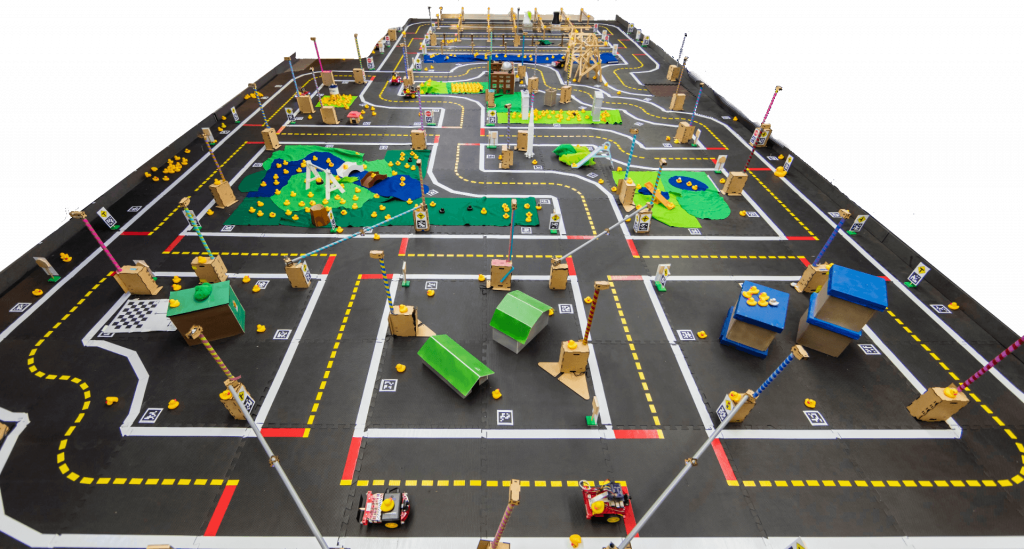
\includegraphics[width=.8\textwidth]{duckietown_exemplo}
	\caption{Exemplo de Duckietown.\label{fig:duckietown_exemplo}}
\end{figure}


\unnumberedsection{Gym-Duckietown}

Este trabalho utiliza o simulador Gym-Duckietown\index{gym-duckietown}~\citep{gym-duckietown} para o treino e execução do veículo autônomo. Esse simulador do universo de Duckietown teve seu início em 2018, dentro do ecossistema Gym desenvolvido pela OpenAI\index{1606.01540}~\citep{1606.01540}, como parte do trabalho feito pelo \textit{Mila - Quebec AI Institute} e com o passar do tempo o projeto evoluiu para um simulador de direção autônoma completamente funcional que pode ser usado para treinar e testar sistemas de aprendizado de máquina além dos algoritmos clássicos da robótica como árvores de decisão ou veículos de \textit{Braitenberg}. Por último o, Gym-Duckietown possui diversas ferramentas para recriar complicações reais, como distorção de câmera, além de aleatorização de domínio para evitar o \textit{overfit} do modelo ao simulador.

\begin{figure}
	\centering
	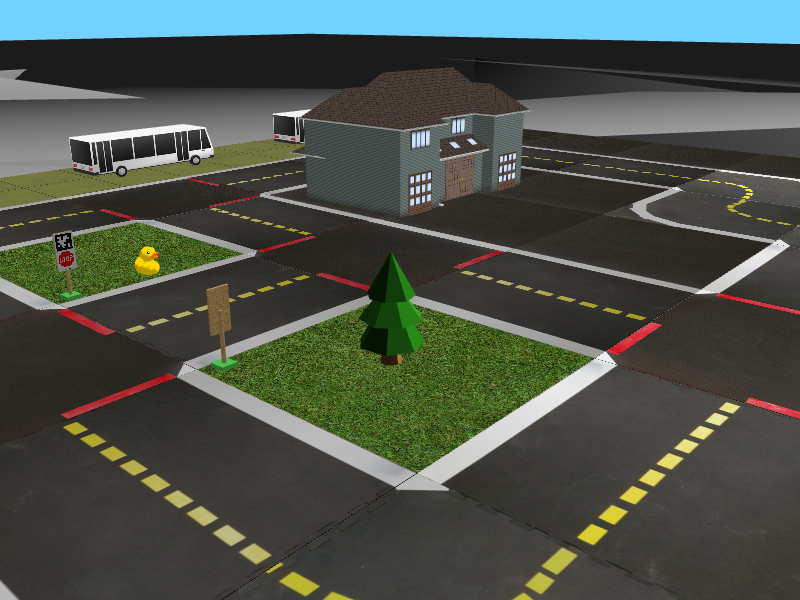
\includegraphics[width=.8\textwidth]{simulador_exemplo}
	\caption{Imagem do Simulador.\label{fig:simulador_exemplo}}
\end{figure}


